\subsubsection*{A. Ayat and the film}

\problemofferer{ Баев А.Ж.}

Ограничения на количество элементов массива позволяют написать наивное решение.

Асимптотика: $O(n)$.



\subsubsection*{B. Big dipper} 

\problemauthor{Баев А.Ж.}

Если второе число меньше первого, то вывести сумму и разность чисел, записанные слитно, иначе вывести 0. 

Асимптотика: $O(1)$.



\subsubsection*{C. Comparing} 

\problemauthor{Баев А.Ж.}

Если количество букв $a$ в первой и второй строке различаются, то привести строки нельзя, иначе можно. Отметим позиции букв $a$ в первой строке $x_1$, $x_2$, ..., $x_n$, позиции букв $a$ во второй строке $y_1$, $y_2$, ..., $y_n$. Ответом на задачу будет:
$$|x_1 - y_1| + |x_2 - y_2| + ... + |x_n - y_n|.$$

Асимптотика: $O(N)$.



\subsubsection*{D. Dima’s divided numbers} 

\problemauthor{Баев А.Ж.}

Необходимо найти минимальное $K$ такое, что $K^M$ делится на $D$. Для этого найдем разложение числа $D$ на простые множители: $$D = p_1^{\alpha_1} p_2^{\alpha_2} ... p_s^{\alpha_s}$$
Сделать это можно за $O(\sqrt{D})$ делений. Ясно, что минимальное $K$ будет вида $p_1^{\beta_1} p_2^{\beta_2} ... p_s^{\beta_s}$, где $\beta_i M \geqslant \alpha_i$. Причем $\beta_i$ должно быть минимально возможное, то есть $\beta_i = \left \lceil \alpha_i / M \right \rceil$.

Асимптотика: $O(\sqrt{D})$.



\subsubsection*{E. Elegant system} 

\problemauthor{Баев А.Ж.}

Рассматривая число как строку $s$ длины $n$ слева направо, найдем первую цифру, отличную от 0 и 1 (обозначим соответствующую позицию $k$). 

Если $s[k-1] = 0$ и число, образованное подстрокой $s[k:n]$, больше $555...55$ ($n-k+1$ цифр 5), то применим округление вверх: заменим $s[k:n]$ на нули и прибавим единицу к числу $s[1:k-1]$ (длинная арифметика). В противном случае, применим округление вниз: заменим все цифры подстроки $s[k:n]$ на нули.

Асимптотика: $O(n)$.



\subsubsection*{F. Fantastic chess}

\problemofferer{ Баев А.Ж.}

Обозначим $d[i][j] = 1$ выигрышной позицией, если начинающий с этой позиции игрок при правильной игре выигрывает, $d[i][j] = 0$ --- проигрышной позицией, в противном случае. Просчитаем $d[i][j]$ для всех $i$ от $N$ до $1$ и $j$ от $M$ до $1$ (порядок вычисления определен с учетом допустимых ходов ферзя). Для каждого $d[i][j]$ просмотрим все допустимые ходы:
\begin{itemize}
\item $d[i+k][j]$, при $k$ от $1$ до $\min(N-i, z)$, где $z$ минимальное такое, что $a[i+z][j] = \text{'x'}$;
\item $d[i][i+k]$, при $k$ от $1$ до $\min(M-j, k)$, где $z$ минимальное такое, что $a[i][j+z] = \text{'x'}$;
\item $d[i+k][j+k]$, где $k$ от $1$ до $\min(N-i, M-j, k)$, где $z$ минимальное такое, что $a[i+z][j+z] = \text{'x'}$;
\end{itemize} 
Если среди допустимых позиций все выигрышные, то данная позиция проигрышная, иначе она выигрышная. Ответ определяется от $d[1][1]$.

Асимптотика: $O(n \; m \max(n,m))$.



\subsubsection*{G. Geometry} 

\problemauthor{Баев А.Ж.}

\begin{center}
\definecolor{light}{rgb}{0.85,0.85,0.85}
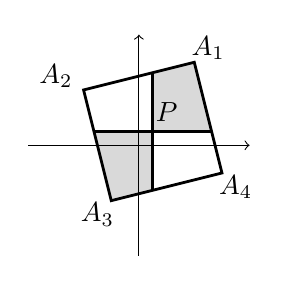
\begin{tikzpicture}[x=10, y=10]
\begin{scope}
	\clip (2, 3) -- (-2, 2) -- (-1, -2) -- (3, -1) -- cycle;
	\fill[fill=light] (0.5, 0.5) -- (0.5, 5.0) -- (5.0, 0.5);
\end{scope}
\begin{scope}
	\clip (2, 3) -- (-2, 2) -- (-1, -2) -- (3, -1) -- cycle;
	\fill[fill=light] (0.5, 0.5) -- (0.5, -5.0) -- (-5.0, 0.5);
\end{scope}
\begin{scope}
	\clip (2, 3) -- (-2, 2) -- (-1, -2) -- (3, -1) -- cycle;
	\draw [line width=1pt] (0.5, -5.0) -- (0.5, 0.5) -- (-5.0, 0.5);
	\draw [line width=1pt] (0.5, 5.0) -- (0.5, 0.5) -- (5.0, 0.5);
\end{scope}

\draw[->] (-4, 0) -- (4, 0);
\draw[->] (0, -4) -- (0, 4);
\draw[line width=1pt]  (2, 3) -- (-2, 2) -- (-1, -2) -- (3, -1) -- cycle;

\node at (2.5, 3.5) {$A_1$};
\node at (-3, 2.5) {$A_2$};
\node at (-1.5, -2.5) {$A_3$};
\node at (3.5, -1.5) {$A_4$};
\node at (1, 1.2) {$P$};
\end{tikzpicture}
\end{center}

Обозначим $A_i(x_i, y_i)$ --- четыре точки в соответствующих четвертях. Фиксируем точку $P(a, b)$, через которую пройдут разрезы $x = a$ и $y = b$. Чтобы определить площади четырех частей, достаточно: найти точки пересечения прямой $x = a$ с отрезками $A_1A_2$ и $A_3A_4$, точки пересечения $y = b$ с отрезками $A_1A_4$ и $A_2A_3$ и вычислить площадь всех четырех частей $S_1$, $S_2$, $S_3$, $S_4$ (площадь четырехугольника вычисляется как площадь двух треугольников). 

Осталось заметить, что величины $S_1 + S_2$ и $S_3 + S_4$ зависят только от $b$ (не зависят от $a$), причем являются монотонными функциями от $b$. Подобрать такое значение $b$, чтобы $S_1 + S_2 = S_3 + S_4$ можно бинарным поиском на отрезке $[\max(y_3, y_4); \min(y_1, y_2)]$. Аналогично подбирается $a$.

Асимптотика: $O(\log(\max(X_i, Y_i) - \min(X_i, Y_i)))$.



\subsubsection*{H. Ha-ha-ha} 

\problemauthor{Баев А.Ж.}

Запустим обход в глубину (или в ширину) с 4 переходами до соседей: $(\pm 1, 0)$ и $(0, \pm 1)$. Если при обходе получилось дойти до ускорителя, то запустим еще один обход но с 8 переходами: $(\pm 1, 0)$, $(0, \pm 1)$, $(\pm 2, 0)$ и $(0, \pm 2)$.

Асимптотика: $O(n m)$.